
The concept of one variable being a function of another is central to the study of most modern pure and applied mathematics. The idea of a function allows us to bring together all the equivalent forms of an expression and solving algebraic equations under one unifying concept. It also provides us with new ways of visualizing algebraic processes via graphs of functions. In this chapter we will explore the different ways of thinking about functions.


\section{Inputs and Outputs}

A \it{function}\normalfont\ is a relation between two variables $x$ (the input) and $y$ (the output) where each input is related to only one output (the variables $x$ and $y$ are generic, different letters may be used). Because this is an algebra course, most such relations will be defined with an algebraic equation with $y$ alone on one side and some algebraic expression involving $x$ on the other. We use letters to name functions; often $f$ is used if we are giving a name to a function when $f$ isn't already in use elsewhere in the problem. If $y$ is related to $x$ by the function $f$ we write
\[
y = f(x).
\]
We read this as ``$y$ equals $f$ of $x$''. 

\subsection{Evaluating Functions and Using Function Notation}

For most people, more needs to be said about how to think about functions and use function notation than was given above. Suppose we are given the definition of a function as
\[
y = f(x) = \mbox{some expression involving } x.
\]
From a symbolic point of view we may think of $f$ as a certain type of shorthand.

\begin{center}
Function Notation as Shorthand 
\begin{tabular}{|p{1.5in} c p{2in} |}
\hline\hline \it{Function: $y = f(x)$} & $\longrightarrow$ & \it{$f(x)$ is a compact way of writing what may be a complicated algebraic expression. }\normalfont\\
\hline
\end{tabular}
\end{center} 

{\bf Remark:} Not all functions are defined using algebraic expressions. For instance trigonometric functions can only be defined using geometry and/or concepts from calculus. However, for our purposes right now, this is an effective way to think about functions.

\par

Because we can think of algebraic expressions as processes carried out on  variables, we may also think of a function as a process performed on $x$, resulting in $y$. Equipped with the idea of equivalence of algebraic expressions, we may think of a function $f$ in a more conceptual way. We can think of $f$ as a factory that takes $x$'s as raw ingredients and makes specific $y$'s. Equivalence of the defining expressions for $f$ can be thought of as rearranging the factory, but ultimately leaving the product being produced unchanged.

\begin{center}
Function as ``$y$ factory'' 
\begin{tabular}{|p{1.5in} c p{2in} |}
\hline\hline \it{Function: $y = f(x)$} & $\longrightarrow$ & \it{$f$ is the set of all processes that result in the same outputs ($y$'s) as the expression $f(x)$. In other words, any expression that is equivalent to $f(x)$ defines the same function, so we say it is also $f(x)$. }\normalfont\\
\hline
\end{tabular}
\end{center} 

In applications, we usually think of the input as a variable we control and the output as one that results from a process. For this reason we call the input the \it{independent variable}\ \normalfont and the output the \it{dependent variable}.
\normalfont

\par

Given a function, you evaluate by plugging in the input for $x$. The result is the value of $y$ corresponding to that $x$-value. 

\par 

\begin{eg} Define the function $f$ by $y = f(x) = 3x^2-1$. Evaluate the following:
\begin{enumerate}
\item[a.] $f(2)$ 
\item[b.] $f(x+1)$ 
\item[c.] $2f(x) -1$
\end{enumerate}
\underline{Solutions:}
\begin{enumerate}
\item[a.]  The function $f(x)$ tells us to take any input $x$ and do the following:  square the input $x$; then multiply by $3$; then subtract $1$.  If $x=2$, we will get:  $2^2 = 4$;  then multiply by $3$ to get $12$; then subtract $1$ to get $11$.  So  $f(2) = 3\cdot 2^2 -1 = 11$.  The output of $f$ when $x=2$ is $y = 11$.
\item[b.] This time,  we think of $x+1$ as our input, a quantity that must be evaluated before $f$ is applied, so we enclose it in parentheses in the evaluation. Then we apply the steps and simplify by expanding and collecting like terms.
\begin{eqnarray*}
f(x+1) & = & 3(x+1)^2 - 1\\
 & = & 3(x^2+2x+1) - 1   \phantom{ww} \textup{ square } (x+1) \\
 & = & 3x^2+6x +3 - 1   \phantom{www} \textup{ multiply by  } 3 \\
  & = & 3x^2+6x + 2.   \phantom{wwwww} \textup{ subtract } 1 \\
\end{eqnarray*}
Note that $f(x+1)$ is not the same function as $f(x)$; for any $x$-value, $f(x+1)$ says that we add $1$ to $x$ and then apply all the steps of $f$.   This can be used to define another function, say $y = g(x) = f(x+1)$.
\item[c.] In this part we first apply $f$ to $x$, and then do two additional steps:   multiply by $2$ and then subtract $1$. Here we think of $f(x)$ as being enclosed in parentheses:
\begin{eqnarray*}
2f(x) - 1 & = & 2(3x^2-1) -1   \phantom{ww} \textup{ apply  } f \textup{ to } x \\
 & = & 6x^2-2-1   \phantom{wwww} \textup{ multiply by  } 2 \\ 
  & = & 6x^2-3.   \phantom{wwwwww} \textup{ subtract   } 1\\
\end{eqnarray*}\qed 
\end{enumerate}
\end{eg}
\par

\begin{question} Let $f(x) = \frac12 x^2$.  Find simplified expressions for each of the following, and describe the steps they represent.

\begin{enumerate}
    \item[a.] $f(3x+2)$
    \item[b.] $3f(x) + 2$
\end{enumerate}
\end{question}



\begin{question} Let $f(x) = x^2-4x+5$ and $g(x) = x^2+1$. Define another function $h(x)$ by saying $h(x) = g(x-2)$. Use algebra to show that $h(x)$ is actually the same function as $f(x)$.
\end{question}

\par

{\bf Domain} One important question about any given function is, ``What are its allowable inputs?" Using the factory analogy, what raw ingredients can that factory work with? This set of numbers is called the \it{domain }\normalfont of the function. One of the primary goals of Calculus is to investigate how functions behave at inputs ``at the boundary'' of the domain. In order to determine the domain of a function, it is good to read through it as a sequence of procedures, then decide if anything is not allowed at any point in that process. Those values of $x$ that force us into an operation that is not allowed with normal arithmetic are the values of $x$ that are \underline{not} \normalfont in the domain.  For functions defined algebraically, the main things that are not allowed are:
\begin{itemize}
\item division by zero, and
\item even roots of negative numbers.
\end{itemize}


\begin{eg}
Suppose we have the function $f(x) = \sqrt{x-2}$.  We want to find the domain.  We see that there is a square root, and so we cannot put a negative value under the square root sign;  thus $x-2$ must be nonnegative.  Set $x-2 \geq 0$, we can solve this to find $x \geq 2$.  Thus the domain is $[2, \infty)$.  
\end{eg}


\begin{eg} Suppose we wish to find the domain of
\[
f(x) = \frac{\sqrt{x^2-1}}{2x+3}.
\]
This function has two main parts:
\begin{enumerate}
\item[\bf Part 1:] Takes the square root of $x^2-1$, then
\item[\bf Part 2:]  Divide {\bf Part 1} by $2x+3$.
\end{enumerate}
We can look at each part separately to determine the domain. For {\bf Part 1}, we can certainly square any  $x$, and subtract $1$.  It is the square root that will be a problem.  We need to have $x^2-1 \geq 0$.   If $x$ is between $-1$ and $1$, then $x^2$ is less than $1$, so $x^2-1$ is negative. So $-1<x<1$ must be excluded from the domain since these values would force us to take the square root of a negative number. For {\bf Part 2},  we are not allowed to divide by zero.  We will find where $2x+3$ is zero and exclude it:   $x=-\frac{3}{2}$. Thus the domain is all $x$ with $x\leq -1$ or $x\geq 1$, except for $x=-\frac{3}{2}$. In interval notation, this would be written as
\[
\left(-\infty,-\frac{3}{2}\right)\bigcup \left(-\frac{3}{2},-1\right] \bigcup \left[1,\infty\right).
\]     
\qed \end{eg}

\begin{question} Find the domain of each of the following functions. {\bf Carefully explain how you found it, as illustrated in the previous example.} Express your answer using inequalities and words, as well as using interval notation (see refresher after the question if you don't remember interval notation).
\begin{enumerate}
\item[a.] $f(x) = \sqrt{3x + 1-x}$
\item[b.] $g(x) = \dfrac{1}{x^2-x-6}$
\item[c.] $h(x) = \dfrac{1}{\sqrt{x^2-x-6}}$
\item[d.] $k(x) = f(x+1)$, where $f$ is the function defined in part (a)
\end{enumerate}
\end{question}

\begin{tcolorbox}
{\bf Interval Notation}\\
\begin{tabular}{p{2in} | p{1.2in} | p{1in}}
Verbal Description & Inequalities Describing $x$ & Interval(s) Containing $x$\\
\hline\hline $x$ is greater than $a$ & $x>a$ & $(a,\infty)$\\
\hline $x$ is greater than or equal to $a$ & $x\geq a$ & $[a,\infty)$\\
\hline $x$ is less than $a$ & $x<a$ & $(-\infty,a)$\\
\hline $x$ is less than or equal to $a$ & $x\leq a$ & $(-\infty,a]$\\
\hline $x$ is greater than (or equal to) $a$ and less than (or equal to) $b$ & $a<(\leq) x <(\leq) b$ & $(a,b),(a,b],[a,b)$, or $[a,b]$,  depending on strictness\\
\hline $x$ is greater than (or equal to) $b$ or less than (or equal to) $a$ & $x>(\geq) b$ or $x<(\leq) a$ & $(-\infty,a)\bigcup(b,\infty)$, with $(,),[,$ or $]$ used at $a$ and $b$, depending on strictness.  
\end{tabular}

\end{tcolorbox}

\begin{question} Sometimes the context of a problem restricts the domain of a function when the algebra may not. For instance, suppose a farmer wants to fence off a rectangular area with three sides of a rectangle, using a river as the fourth side. He has 100 yards of fence to use. Let $x$ denote the length of the side of the rectangle parallel to the river. Find a formula for the function $A(x)$ that gives the area as a function of $x$. What is the domain of this function based on the formula and what is it based on the context of the problem? 
\end{question}

\subsection{Solving Equations Involving Functions}

In solving algebraic equations, perhaps the most straightforward ones to solve are of the form
\[
(\mbox{algebraic expression}) = \mbox{a number},
\]
where the algebraic expression on the left represents a process applied to a variable that we reverse to solve. Equipped with the idea of functions, we now can simply think of these in the form 
\[
f(x) = \mbox{a number}.
\] 
More complicated equations typically have the form
\[
f(x) = g(x),
\]
where $f$ and $g$ are different functions. When we think of function notation as shorthand for specified algebraic expressions, solving equations involving functions is not different than solving equations as we have before now. 

\par 

\begin{eg} Let $f(x) = x^2-3x$ and $g(x) = 2x-4$. Let's solve the following equations;
\begin{enumerate}
\item[a.] $g(x) = 8$
\item[b.] $f(x) = g(x)$
\item[c.] $f(x+1) = g(x)$
\end{enumerate}
\underline{Solutions:}
\begin{enumerate}
\item[a.] . For (a) we use the fact that $g(x) = 2x-4$, so  we get the following:
\begin{eqnarray*}
2x-4 & = & 8\\
& \updownarrow &\\
2x& = & 12\\ 
& \updownarrow &\\
x& =& 6.
\end{eqnarray*}
\item[b.] For (b), we use $f(x) = x^2-3x$ and $g(x) = 2x+4$.  Then we factor to solve: 
\begin{eqnarray*}
x^2 - 3x  & = & 2x-4\\
& \updownarrow & \\
x^2-5x+4 & = & 0\\
& \updownarrow & \\
(x-4)(x-1) & = & 0\\
& \updownarrow & \\
x=4 & \mbox{or} & x=1.
\end{eqnarray*}
\item[c.] For (c), we need to figure out what $f(x+1)$ means.  Now $f$ is the function that takes any input, squares it, then  multiplies a new copy of it by three, then finds the difference. In this case, our input is the quantity $(x+1)$. So we to is substitute $(x+1)$ each time we see and $x$ in the expression for $f(x)$ and set it equal to $g(x)$:
\begin{eqnarray*}
(x+1)^2 - 3(x+1) & = & 2x-4\\ 
& \updownarrow & \mbox{expand, group like terms on one side}\\
x^2-3x+2 & = & 0\\
& \updownarrow & \\
(x-1)(x-2) & = & 0\\
& \updownarrow & \\
x=1 & \mbox{or} & x=2.
\end{eqnarray*}
\end{enumerate}
\qed \end{eg}

\par
\begin{question}
Let $f(x) = x-1$, and $g(x) = (x-3)^2$.  Solve each of the following equations:
\begin{enumerate}
\item[a.] $f(x) = 2$
\item[b.] $f(x) = 2x-6$
\item[c.] $f(x) = g(x)$
\end{enumerate}
\end{question}


\begin{question} Let $f(x) = \dfrac{x}{3x+7}$. Solve the following equations, if possible. If it is impossible to solve, explain why.
\begin{enumerate}
\item[a.] $f(x) = 1$
\item[b.] $f(x) = x$
\item[c.] $f(x) = \frac{1}{3}$
\end{enumerate}
\end{question}

As seen in part (c) of the last question, some numbers may not appear as outputs of a given function. The set of numbers that \it{do} \normalfont appear as outputs of a given function is called the \it{range} \normalfont of the function. Another way to say what the range of $f$ is, is that it is the set of $y$ such that there is a solution to the equation $y=f(x)$. Finding the range of a function is generally a more difficult task than finding its domain; being able to find the maximum and/or minimum possible outputs of a given function is one of the main achievements of Calculus. However, in many cases we can determine the range of an algebraically defined function by some combination of the following:
\begin{itemize}
\item Determine what arithmetic operations the function applies to its input, and think about what the possible results could be.
\item Solve the general equation $y=f(x)$ for $x$, if possible. The result will be an expression involving $y$; the range of $f$ will be the $y$-values that can be substituted into this expression.
\end{itemize} 

\begin{eg} Find the range of the following functions:
\begin{enumerate}
\item[a.] $f(x) = \dfrac{x}{3x+7}$
\item[b.] $g(x) = -(x-3)^2 + 4$
\item[c.] $h(x) = 2x+1$
\item[d.] $k(x) = 2x+1 + \sqrt{x-1}$
\end{enumerate}
\underline{Solutions:} 
\begin{enumerate}
\item[a.] This is the function from Question 4.10. If we solve the equation
\[y = \frac{x}{3x+7}\]
for $x$, we have the general solution
\[
x = \frac{7y}{1-3y}.
\]
The only $y$-value that cannot be substituted into this is $y=\frac{1}{3}$. Thus, the range of $f$ is all real numbers except $\frac{1}{3}$. Using inequalities, we would write $y<\frac{1}{3}$ or $y>\frac{1}{3}$. In interval notation, it would be written as $\left(-\infty,\frac{1}{3}\right)\bigcup\left(\frac{1}{3},\infty\right)$. 

\par

{\bf Remark:} For problems involving domain and range, using inequalities to describe the domain and range may be preferable to interval notation. This is because inequalities make explicit which variables are elements of the domain (the input variable) and the range (the output variable).

\item[b.] For this problem, we can use our understanding of the defining expression to find the range. The function $g$ takes $x$ and subtracts three from it, squares the result, multiplies that by $-1$, and finally adds four. Noting that squares are never negative, $-(x-3)^2$ will never be positive. This means no positive number is ever added to four. A little thought shows that any number less than or equal to four is an output of this function. So the range is $y\leq 4$.

\item[c.] Algebraically solving $y=h(x)$ for $x$ yields $x = \frac{y-1}{2}$. No values of $y$ make the right-hand side of this equation undefined, so the range is $-\infty < y < \infty$.

\item[d.] For this problem, we must note the domain of the function before determining the range. Because of the inclusion of the $\sqrt{x-1}$ term, the domain of $k$ is $x\geq 1$. Possible outputs of $2x+1$ over this domain are all numbers greater than or equal to three. Putting this together with the possible outputs of the expression $\sqrt{x-1}$, we see the range of $k$ is $y\geq 3$.
\end{enumerate}
\qed \end{eg}  

\begin{question} Determine the domain and range of the following functions. Explain your answers carefully as in the last example.
\begin{enumerate}
\item[a.] $f(x) = -2(x-4)^2+3$
\item[b.] $g(x) = \dfrac{1}{\sqrt{x-4}}$
\end{enumerate}
\end{question}     



\section{Graphs of Functions}

Until now, our development has regarded a function as only slightly different than an algebraic expression. Algebraic expressions represent processes applied to their variables (the inputs), just like functions. The function concept blends this idea with solving equations by considering the evaluation result (the output) as a key piece; the output is a number that the function can equal for some input, which may be solved for. The graph of a function takes us a step further, so that we may see the totality of all inputs and outputs of the function as a single object, the graph of the function.

\par

The graph of a general function of the form $y = f(x)$ is a set of points in the $xy$-plane (or whatever the input and output variables happen to be). To plot a single point $(a,b)$ in the $xy$-plane, we move a distance of $a$ along the $x$-axis (the horizontal axis), then a vertical distance $b$ from there (the vertical axis is the $y$-axis as in the following figure:

\begin{figure}[h]
\centering
\begin{tikzpicture}[yscale=1]
\draw[thick] [<->] (-1,0) -- (5,0);
\draw[thick] [<->] (0,-1) -- (0,5);
\draw (2,-.1) -- (2,.1);
\draw (-.1,1) -- (.1,1);
\node[align=center,below] at (2,0){$a$};
\node[align=center,left] at (0,1){$b$};
\node[align=center,below] at (5,0){$x$};
\node[align=center,left] at (0,5){$y$};
\draw [fill] (2,1) circle [radius=0.05];
\node[align=center,right] at (2,1){$(a,b)$};
\end{tikzpicture} 
\caption{A typical point in the $xy$-plane.}
\end{figure}

\begin{tcolorbox}
{\bf The Graph of a Function}\\
The graph of $y = f(x)$ is the set of all points in the $xy$-plane that satisfy the equation $y=f(x)$. Stated another way we have the following equivalence:
\[
(a,b)\ \mbox{is on the graph of\ }\\ y=f(x)\ \mbox{if and only if}\ b = f(a).
\]
\end{tcolorbox}
To sketch the graph of a function, one starts by finding a reasonable number of points on the graph, often putting them in an input-output table, then plotting them in the plane. When a general pattern is evident, we usually fill in between the plotted points with a smooth curve.

\par

\begin{eg} Consider the function $y = f(x) = x^2-4$. First, we will find some pairs of points on the graph by evaluating the function for some $x$-values and recording the results in a table:\\
\begin{center}
\begin{tabular}{c || r|r|r|r|r|r|r|}
$x$ & $-3$ & $-2$ & $-1$ & $0$ & $1$ & $2$ & $3$ \\ 
\hline $y = f(x) = x^2-4$ & $5$ & $0$ & $-3$ & $-4$ & $-3$ & $0$ & $5$\\
\hline
\end{tabular}
\end{center}

Then we plot the points according to the table and fill in a curve: \\

\begin{figure}[h]
\centering
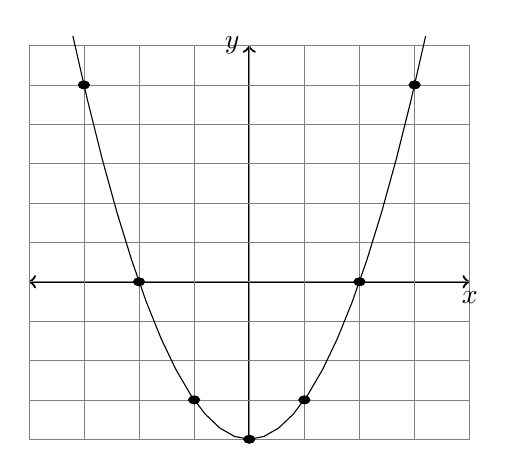
\begin{tikzpicture}[xscale=.7,yscale=.5]
\draw[thick] [<->] (-4,0) -- (4,0);
\draw[thick] [->] (0,-4) -- (0,6);
\draw [help lines] (-4,-4) grid (4,6);
\node[align=center,below] at (4,0){$x$};
\node[align=center,left] at (0,6){$y$};
\draw [fill] (-3,5) circle [radius=0.1];
\draw [fill] (-2,0) circle [radius=0.1];
\draw [fill] (-1,-3) circle [radius=0.1];
\draw [fill] (0,-4) circle [radius=0.1];
\draw [fill] (3,5) circle [radius=0.1];
\draw [fill] (2,0) circle [radius=0.1];
\draw [fill] (1,-3) circle [radius=0.1];
\draw [domain=-3.2:3.2] plot (\x, {\x*\x-4});
\end{tikzpicture} 
\caption{The graph of $y = x^2-4$.}
\end{figure}

\qed \end{eg}


\begin{question} On your own paper, carefully graph the following functions by plotting at least six points.
\begin{enumerate}
\item[a.] $f(x) = 3x-2$
\item[b.] $g(x) = \sqrt{x}$
\item[c.] $h(x) = \dfrac{1}{x}$ (Be sure to plot several points with $x$ values between $-1$ and $1$.)
\end{enumerate} 
\end{question}

Equipped with graphs of functions, we may now catalog graphical interpretations of many of the skills and concepts we have encountered so far.

\begin{tcolorbox}
{\bf Graphical Interpretations of Algebraic Skills with Functions}
\begin{itemize}
\item To evaluate a function at some value $x=a$, move to the $a$ position on the horizontal axis and then find the vertical coordinate on the graph above or below that point.
\item To solve an equation of the form $f(x) = b$, find the $x$-coordinates of all points on the graph whose $y$-coordinate is $b$.
\item To solve an equation of the form $f(x) = g(x)$, we are asking for the input values such that $f$ and $g$ give the same output. Hence we must find the $x$-coordinates of all points of intersection between the graphs of $f$ and $g$. 
\item The domain of a function is the set of $x$-coordinates of all points on the graph. This may be visualized as the set of values on the horizontal axis that lie above or below the graph of the function.
\item The range of a function is the set of $y$-coordinates of all points on the graph. This may be visualized as the set of values on the vertical axis that lie to the left or right of the graph of the function.
\end{itemize}
\end{tcolorbox}

\pagebreak

\begin{question} Consider the graph of the function shown below (the \underline{entire}\ \normalfont graph is shown).\\
\begin{figure}[h]
\centering
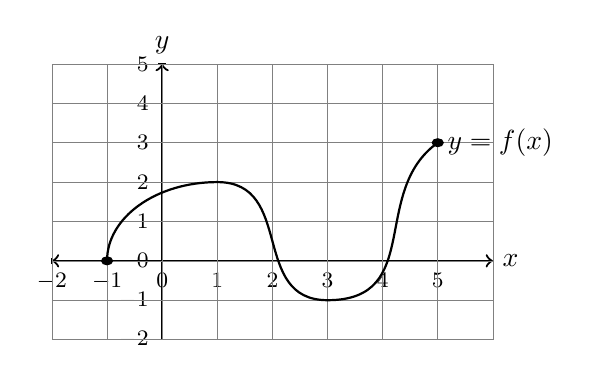
\begin{tikzpicture}[xscale=.7,yscale=.5]
\foreach \x in {-2,-1,0,1,2,3,4,5}\draw[shift={(\x,0)},color=black] (0pt,2pt) -- (0pt,-2pt) node[below] {\footnotesize $\x$};
\foreach \y in {-2,-1,0,1,2,3,4,5}\draw[shift={(0,\y)},color=black] (2pt,0pt) -- (-2pt,0pt) node[left] {\footnotesize $\y$};
\draw[thick] [<->] (-2,0) -- (6,0);
\draw[thick] [->] (0,-2) -- (0,5);
\draw [help lines] (-2,-2) grid (6,5);
\node[align=center,right] at (6,0){$x$};
\node[align=center,above] at (0,5){$y$};
\node[align=center,right] at (5,3){$y=f(x)$};
\draw [fill] (-1,0) circle [radius=0.1];
\draw [fill] (5,3) circle [radius=0.1];
\draw[thick] (-1,0) to [out=90,in=180] (1,2)
to [out=0,in=180] (3,-1) to [out=0,in=225] (5,3) ;
\end{tikzpicture} 
\end{figure}
Find each of the following, approximate if necessary:
\begin{enumerate}
\item[a.] The domain of $f$.
\item[b.] The range of $f$.
\item[c.] $f(1)$
\item[d.] All solutions to the equation $f(x) = 1$.
\item[e.] All solutions to the equation $f(x) = x+1$.
\end{enumerate}
\end{question} 


\section{Composite and Inverse Functions}

On many occasions we have broken down algebraic expressions as a sequence of steps, often determined by order of operations. Now that we have the concept of a function, we may view this breaking down in terms of \it{function composition or decomposition}.\ \normalfont Simply put, we may view each step in a sequence of operation defining a function as its own function. For instance, consider the function $h$ defined by the algebraic expression in the first example of Chapter 2. This function is 
\[
 y =  h(x) = (3x+1)^2-2.
\]
When we broke down that expression, we noted that it takes $x$ and does the following:  
\begin{enumerate}
\item[\bf S1:] multiplies $x$ by $3$, 
\item[\bf S2:] adds one to {\bf S1}
\item[\bf S3:] squares {\bf S3},  and finally
\item[\bf S4:] subtracts two from {\bf S4}, 
\end{enumerate}
to give us an output $y$. Now, we can think about this as two processes, one that does the first two steps {\bf S1} and {\bf S2}, and one that does the last two steps {\bf S3} and {\bf S4}.   For the first two steps, we can use the function 
\[
u = g(x) = 3x+1.
\]
The last two steps then are performed on the output of $g$ by another function
\[
y = f(u) = u^2-2.
\]
Symbolically, we substitute the expression for $g(x)$ into $f(u)$ for $u$ to get our expression for $h(x)$:
\[
y = h(x) = f(g(x)).
\]
In general, a new function $h$ constructed out of a pair of functions $g$ and $f$ is called the \it{composition of $f$ with $g$}.\normalfont\ The function $g$ is referred to as the \it{inside\ }\normalfont function and $f$ is referred to as the \it{outside\ }\normalfont function. The inputs of the composition are the inputs of the inside function and the outputs are the outputs of the outside function. 

\par

\begin{question} If $u = f(x) = 2+3x$ and $x=g(u) = 5u+1$, then both $f(g(u))$ and $g(f(x))$ make sense. Find them. Are they the same?
\end{question}

\par 

\begin{eg} Often we decompose functions by finding inside and outside functions that are easier to work with than the composite. One task that we do this for is finding domains and ranges of composites. For instance, consider the function
\[
y = \sqrt{x^2-1}.
\]
This may be decomposed as $f(g(x))$ where $u = g(x) = x^2-1$ and $y=f(u) = \sqrt{u}$. The domain of the composite is those inputs of the inside function that, when the inside function is applied, result in legal inputs of the outside function. The domain of the outside function is $u\geq 0$, hence we must find $x$'s such that the output of $x^2-1$ is non-negative. This occurs only if $x\geq 1$ or $x\leq -1$ as numbers between $-1$ and $1$ will square to something less than one. Thus the domain is $x\leq -1$ or $x\geq 1$. The outputs of $u = x^2-1$ over this domain are all $u\geq 0$, thus the entire range of $\sqrt{u}$ will be covered. Thus the range of $y = \sqrt{x^2-1}$ is all $y\geq 0$.
\end{eg}
\par 

\begin{question} Decompose $y = h(x) = \dfrac{2}{x^2-9}$ as an inside function and outside function and use that decomposition to find the domain of $h$ as in the previous example.
\end{question}

\par 

One important application of the idea of function composition is that of \it{inverse functions.\ }\normalfont In short, the inverse of a given function undoes the action of that function. This leads us to the following formal definition:

\begin{tcolorbox}
{\bf Definition of the Inverse Function}
Given a function $y = f(x)$, the \it{inverse function\ }\normalfont to $f$ is the function $x = f^{-1}(y)$ such that
\[
f^{-1}(f(x)) = x\ \mbox{and}\ f(f^{-1}(y)) = y.
\]
The inputs of the inverse function are the outputs of $f$, the outputs of the inverse function are the inputs of $f$, and the two functions undo one another.
\end{tcolorbox}

\begin{eg}
\begin{enumerate} 
\item[i.] Consider the function defined by the expression
\[
y = f(x) = (x-4)^3 + 3.
\]
By breaking this down into steps (decomposing the function), we are able to sequentially build the inverse function
\[
x = f^{-1}(y) = \sqrt[3]{y-3} + 4.
\]
\item[ii.] In the Equation Practice worksheet, problem 3, we found the inverse of the function
\[
y =g(x) = \sqrt[3]{4x-7}
\]
to be
\[
x = g^{-1}(y) = \frac{y^3+7}{4}.
\]
We then used the inverse function to solve for $x$ given several outputs. In this way, we may think of the inverse of a function as the general equation solving function, provided it's just a number on the opposite side of the equation from the function.
\end{enumerate}\qed \end{eg}

The characterization of an inverse function as an equation solving function allows us to give an algebraic procedure for finding expressions of inverse functions even when we may not see how to reverse the process of the given function; simply write down the equation defining the function $y=f(x)$, and solve for $x$ in terms of $y$.

\par

\begin{question} Find the inverse $f^{-1}(y)$ for the function
\[
y = f(x) = \frac{4-3x}{7-9x}.
\]
\end{question}

The graph of the inverse to a given function has a particularly nice relationship to the graph of its parent function. To graph the inverse to a function $y=f(x)$, simply take the entire picture of the graph of $f$, including axis labels, and reflect it across the line through the origin making a 45 degree angle with the positive $x$ axis.

\begin{figure}[h]
\begin{minipage}[b]{0.5\textwidth}

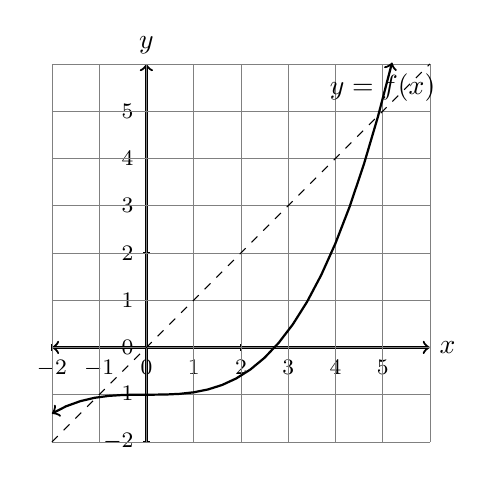
\begin{tikzpicture}[xscale=.6,yscale=.6]
\foreach \x in {-2,-1,0,1,2,3,4,5}\draw[shift={(\x,0)},color=black] (0pt,2pt) -- (0pt,-2pt) node[below] {\footnotesize $\x$};
\foreach \y in {-2,-1,0,1,2,3,4,5}\draw[shift={(0,\y)},color=black] (2pt,0pt) -- (-2pt,0pt) node[left] {\footnotesize $\y$};
\draw[thick] [<->] (-2,0) -- (6,0);
\draw[thick] [->] (0,-2) -- (0,6);
\draw [help lines] (-2,-2) grid (6,6);
\node[align=center,right] at (6,0){$x$};
\node[align=center,above] at (0,6){$y$};
\node[align=center,above] at (5,5){$y=f(x)$};
\draw[thick,<->,domain=-2:5.2] plot (\x, {-1+.05*\x*\x*\x});
\draw[dashed,domain=-2:6] plot (\x,\x);
\end{tikzpicture} 
\end{minipage}
\hfill
\begin{minipage}[b]{0.5\textwidth}
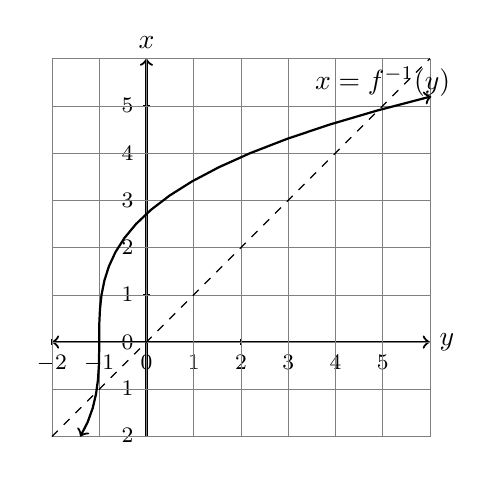
\begin{tikzpicture}[xscale=.6,yscale=.6]
\foreach \x in {-2,-1,0,1,2,3,4,5}\draw[shift={(\x,0)},color=black] (0pt,2pt) -- (0pt,-2pt) node[below] {\footnotesize $\x$};
\foreach \y in {-2,-1,0,1,2,3,4,5}\draw[shift={(0,\y)},color=black] (2pt,0pt) -- (-2pt,0pt) node[left] {\footnotesize $\y$};
\draw[thick] [<->] (-2,0) -- (6,0);
\draw[thick] [->] (0,-2) -- (0,6);
\draw [help lines] (-2,-2) grid (6,6);
\node[align=center,right] at (6,0){$y$};
\node[align=center,above] at (0,6){$x$};
\node[align=center,above] at (5,5){$x=f^{-1}(y)$};
\draw[thick,<->,domain=-2:5.2] plot ({-1+.05*\x*\x*\x},\x);
\draw[dashed,domain=-2:6] plot (\x,\x);
\end{tikzpicture}
\end{minipage}
\caption{The graphs of $y=f(x)$ and $x = f^{-1}(y)$, side by side.}
\end{figure} 
   
\begin{question} Why does it not make sense to graph $f$ and $f^{-1}$ on the same set of axes?   
\end{question} 
   
  
